\chapter{Mission}
\section{Sujet de stage}
Le sujet de mon stage était initialement \texttt{Développement/Intégration de fonctions de Vision par ordinateur pour l’inspection automatisée}. Durant toute la période de mon stage, mon travail s'est axé autour d'un logiciel appelé \texttt{PowerEye}. \texttt{PowerEye} est un logiciel développé pour des scénarios industriels qui utilise la vision par ordinateur pour détecter les défauts des pièces sur la chaîne de production. Les laboratoires de l’UTC faisant partie de ce projet, ils assurent le développement des machines apprenantes. Deltacad est responsable de la conception de l'interface de l'ensemble du projet et de l'intégration des autres fonctions. \\

Avant que je ne commence mon stage, \texttt{PowerEye} avait déjà été conçu avec certaines fonctionnalités ainsi qu'un prototype d'interface. Cependant, il était clair que le système n'était pas encore adapté à une application formelle au sein de l'entreprise. Par conséquent, la tâche principale de mon stage consistait à concevoir et améliorer une interface homme-machine plus pratique basée sur le prototype de l'interface et essayer de tester les pièces d'AML Systems\footnote{un société du segment éclairage du groupe Johnson Electric, conçoit, produit et commercialise, des solutions pour améliorer la visibilité, la sécurité, et le confort du conducteur} à l'aide de cette interface après intégration de la fonction.\\

En ce qui concerne les lignes directrices spécifiques pour la conception de l'interface, le chef de projet et le suiveur m'ont fourni un aperçu général des différents modules qu'elle contiendrait et des fonctionnalités qu'elle pourrait inclure. Après avoir confirmé le thème et le programme de travail, mon stage a officiellement commencé.\\

\newpage
\section{Planning de stage}
Au début de mon stage, mes tâches étaient planifiées en trois phases : 
\begin{itemize}
    \item \textbf{1. }Développement de l'interface homme-machine de PowerEye 
    \item \textbf{2. }Test sur les données de l'entreprise partenaire AML système
    \item \textbf{3. }Déploiement d'applications dans le système AML
\end{itemize}

Dans le cadre du travail réel, pour chaque phase de la tâche, je l'ai décomposée en différentes étapes. La première phase peut en fait être divisée en plusieurs parties : la conception de l'interface, la réalisation de l'apparence de l'interface, la réalisation de la structure des données de l'interface et la réalisation des fonctions de la couche d'application de l'interface. La deuxième phase comprend également l'intégration de la fonctionnalité conçue, le test des données et l'amélioration de la fonctionnalité. Il est très regrettable qu'en raison de contraintes de temps, mon stage se soit terminé à la deuxième phrase. Mais en fait, en plus des tâches incluses dans le plan, j'ai également complété un certain nombre d'autres fonctionnalités, y compris enregistrement des appels de fonction et exécution de programmes de script c\# via des chaînes de caractères\\

À mon avis, la partie la plus importante du processus de stage est la structure globale du projet, car elle influe grandement sur le développement des idées et l'évolutivité du projet. À cette fin, j'ai amélioré l'architecture globale à plusieurs reprises au cours du processus de développement, en utilisant des \texttt{prism} au début de projet individuel, en divisant l'interface en couches d'affichage et d'application, et en développant avec le cadre mvvm.



\newpage
\section{Contributions}
Comme mentionné dans la section précédente, lorsque j'ai commencé à travailler sur le projet, il existait déjà un prototype d'interface ainsi que certains modules fonctionnels.
\begin{figure}[H]
    \centering
    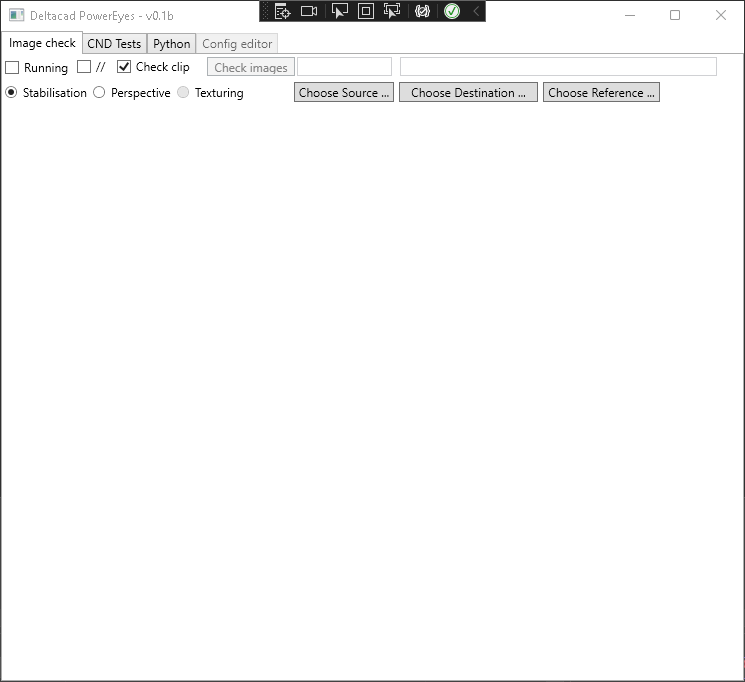
\includegraphics[height=5cm]{ressources/images/prototype.png}
    \caption{Prototype d'interface PowerEye}
\end{figure}
L'interface se compose de quatre modules: Image check, CND Tests, python et config editor. Il contient des méthodes d'application de de Template Matching pour la détection des pièces et des modèles d'entraînement pour les tests avec des ensembles de données.\\
Mais le fait est que l'interface prototype n'est pas suffisante pour inclure toutes les fonctionnalités envisagées par PowerEye. Par conséquent, ma principale contribution tout au long du stage a été la conception et le développement d'une nouvelle version de l'interface \texttt{PowerEye}. À la fin du stage, la nouvelle version de l'interface de powereye ressemblait à ceci. \\
\begin{figure}[h]
    \centering
    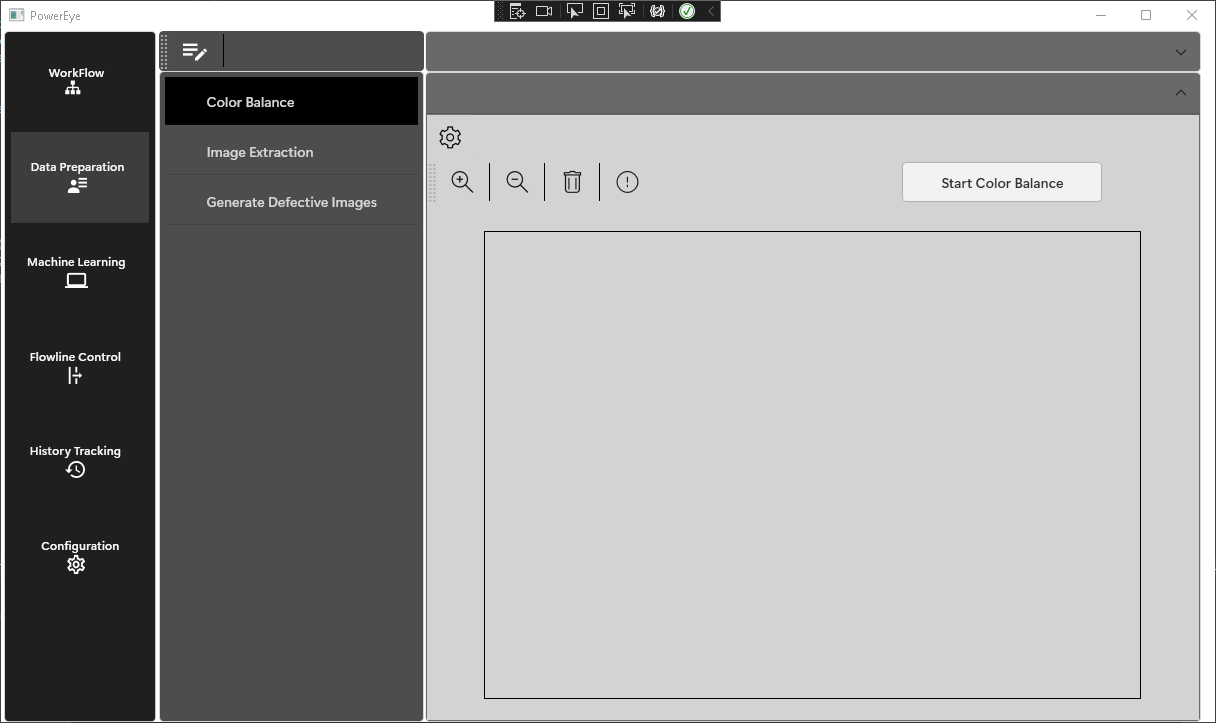
\includegraphics[height=6cm]{ressources/images/color_balance.png}
    \caption{Interface PowerEye redessinée}
\end{figure}
Il contient cinq modules : 
\begin{itemize}
    \item \textbf{Préparation des données (Data preparation): }Ce module permet d'extraire les contours des pièces de l'image et d'ajouter du bruit de perlin à l'image. 
    \item \textbf{Apprentissage automatique (machine learning): }Ce module est utilisé pour entraîner le modèle ckpt à partir de l'ensemble de données.
    \item \textbf{Contrôle de la chaîne d'assemblage (flowline control): } Ce module détecte si une pièce est qualifiée par Template Matching, et enregistre les données du résultat du test.
    \item \textbf{Interroger les données historiques  (History tracking): }Ce module interroge les données du fichier Excel par mots-clés.
    \item \textbf{Configuration des données globales (configuration): }Ce module affiche la configuration complète du logiciel en cours et l'importe par l'intermédiaire de fichiers de configuration.
\end{itemize}

En plus de la partie principale du logiciel, j'ai mis en place les fonctionnalités suivantes
\begin{itemize}
    \item Utilisation du cadre AOP pour afficher les actions de la couche applicative.
    \item Implémentation d'un script c\# qui s'exécute à partir d'une chaîne de caractères.
    \item Implémentation d'ajouts manuels de fonctionnalités existantes pour personnaliser le flux de travail.
\end{itemize}

Ce qui ci-dessus résume essentiellement toutes les contributions que j'ai apportées au cours de mon stage. Dans mon travail, j'ai conçu et développé le projet de manière indépendante en utilisant les exigences comme point de départ, et j'ai finalement bien accompli la tâche. 

\newpage
\section{Outils et technologies}
Tout au long de mon stage, j'ai travaillé avec les outils suivants : 
\begin{itemize}
    \item \textbf{Pour le développement :}
    \begin{itemize}
        \item \textit{Comme langage de programmation :} C\#, WPF.NET, C++, Python 
        \item \textit{Comme environnement de développement :} Microsoft Visual Studio, \gls{IDE}  complet pour les développeurs .NET et C++ sur Windows.
    \end{itemize}
    \item \textbf{Pour la bureautique :} \gls{LaTeX}, pour la rédaction de ce rapport. WebEx, pour les réunions de projet à distance
    \item \textbf{Pour la gestion des différentes versions du logiciel :} \gls{SmartSVN}, un système de gestion des versions.
\end{itemize}

Pour la réalisation du projet, j'ai utilisé les extensions suivantes :
\begin{itemize}
    \item \textbf{WPF-UI :} Extension pour modifier le style du contrôle
    \item \textbf{MahApps.Iconpacks :} Extension pour l'ajout d'icônes de boutons
    \item \textbf{Fody :} Extension pour la mise en œuvre du cadre aop
    \item \textbf{YamlDotNet :} Extension pour les modifications de l'édition yaml
\end{itemize}


\section{Validation de travaux}
La validation de mes travaux se déroulait lors de réunions avec l'équipe de projet. Comme le chef de projet ne travaille pas au même endroit que moi, nos réunions se passaient généralement à distance via le WebEx.

Au cours de la réunion, normalement, je commençais par présenter et démontrer l'état d'avancement de la tâche. Ensuite, le tuteur et le chef de projet discutaient avec moi des améliorations à apporter et planifient les tâches suivantes. le contenu de chaque réunion était enregistré par le chef de projet et m’était envoyé par e-mail après la réunion.

Cela me permet de partager mon point de vue sur le projet et me donne une idée claire de ce qui doit être fait a la phase actuel, ce qui améliore grandement mon efficacité et standardise mon travail.

\newpage
\section{Prise de recul}
\subsection{Intérêt de mon travail}
L'intérêt de mon travail pour l'équipe était de concevoir et développer une IHM plus aboutie que la précédente, migrer et améliorer les fonctionnalités développées précédemment. En outre, le cadre aop et le modèle de l'observateur sont plus propices à la maintenance de l'interface, et il existe un bon cadre général pour le développement du suivi. 

\subsection{Améliorations à envisager}
Mais tout comme le développement de nombreux logiciels connus nécessite beaucoup de polissage, le logiciel que j'ai développés au cours de mon stage de six mois n'étaient certainement pas parfait. Dans le développement futur du projet, les améliorations suivantes sont nécessaires.
\begin{itemize}
    \item Développer la fonctionnalité de certains modules et les intégrer dans l'interface.
    \item Extension de l'utilité de l'interface, par exemple par l'ajout de la touche de raccourci.
    \item Améliorer les fonctionnalités pour s'adapter aux différents produits de l'industrie.
\end{itemize}

\subsection{Réflexions sur l’impact de mon travail}
Selon moi, ma contribution permettra aux utilisateurs de simplifier le processus, de réduire le coût d'apprentissage de l'interface et de rendre la visualisation des résultats plus intuitive.